\subsection{Symmetriegruppen} \label{sec:symmetrieeigenschaftwürfel}

Wir definieren die Symmetriegruppe von einem Polyeder wie folgt
\begin{definition}
Sei $X \subset \mathbb{R}^n$ eine geometrische Figur (in unserem Fall ein Polyeder im $\mathbb{R}^3$). Eine Symmetrie von $X$ ist eine abstandserhaltende Abbildung (Isometrie) $f: \mathbb{R}^n \to \mathbb{R}^n$, die die Figur als Ganzes auf sich selbst abbildet, für die also gilt: $f(X) = X$. Die Symmetriegruppe $S(X)$ ist die Menge all dieser Symmetrien von $X$. Die Gruppenoperation ist dabei die einfache Hintereinanderausführung (Komposition) der Abbildungen.
\end{definition}

\begin{example}[Symmetriegruppe: Reguläres Tetraeder] \label{ex:regulaeres_tetraeder}
Das reguläre Tetraeder hat genau 12 Kongruenzabbildungen. Diese kann man auf mehrere Arten finden. Einerseits wissen wir, dass ein Tetraeder 6 Kanten besitzt, welche in 2 Richtungen orientiert werden können. Daraus folgt, dass es $12$ Abbildungen gibt. Andererseits können wir die Abbildungen auch zählen. 
\begin{center}
\begin{tabular}{ |c|c|c|c| } 
 \hline
 Beschreibung & Symmetrieachse & Periodizität & Anzahl Abbildungen \\ 
 \hline
 Identität & - & - & 1 \\ 
 Ecke, Mitte geg. Dreiecksfläche& K-M & $\frac{\pi}{3}$ & $2*4 = 8$  \\ 
 Kante, Kante& K-K & $\frac{\pi}{2}$ & $1*3=3$  \\ 
 \hline
  & & & 12 \\ 
 \hline
\end{tabular}
\end{center}
\end{example}

\begin{example}[Reguläres Hexaeder] \label{ex:regulaeres_hexaeder}
TODO:...
\end{example}

\begin{example}[Reguläres Ikosaeder] \label{ex:regulaeres_ikosaeder}
TODO:...
\end{example}


\subsubsection{Richtungserhaltende Abbildungen}
\begin{align}
    todo:
\end{align}


\subsubsection{Irreduzibilität}
In diesem Abschnitt untersuchen wir eine grundlegende Eigenschaft der orientierungserhaltenden Symmetriegruppen des regulären Tetraeders, Hexaeders und Ikosaeders. Wir bezeichnen mit $T$ die Gruppe der orientierungserhaltenden Symmetrien (Drehgruppe) des Tetraeders sowie analog mit $H$ und $I$ jene des Hexaeders respektive des Ikosaeders.

\begin{definition}
Sei $V$ ein Vektorraum (in unserem Fall der $\mathbb{R}^3$) und $G$ eine Gruppe von linearen Abbildungen, die auf $V$ operiert. Ein Unterraum $U \subseteq V$ heißt $G$-invariant (oder stabil unter $G$), wenn für jedes Element $g \in G$ und jeden Vektor $u \in U$ gilt, dass das Bild $g(u)$ wieder in $U$ liegt. Die Operation der Gruppe $G$ auf dem Raum $V$ heißt irreduzibel, wenn die einzigen $G$-invarianten Unterräume der triviale Nullraum $\{0\}$ und der gesamte Raum $V$ selbst sind. Gibt es hingegen einen echten invarianten Unterraum (also $U \neq \{0\}$ und $U \neq V$), so nennt man die Gruppe reduzibel.
\end{definition}


\begin{lemma} \label{lemma:irreduzibelsymmetriegruppen}
    Die orientierungserhaltenden Symmetriegruppen des Tetraeders ($T$), Hexaeders ($H$) und Ikosaeders ($I$) operieren irreduzibel auf dem $\mathbb{R}^3$. Das bedeutet, dass unter der Wirkung dieser Gruppen keine nicht-trivialen invarianten Unterräume existieren.
\end{lemma}

\begin{proof}
    Angenommen, eine Gruppe $\Omega \in \{T, H, I\}$ operiere reduzibel auf dem $\mathbb{R}^3$. Dann existiert per Definition ein echter invarianter Unterraum $U \subset \mathbb{R}^3$ der Dimension 1 (eine Gerade durch den Ursprung) oder der Dimension 2 (eine Ebene durch den Ursprung). Invariant bedeutet, dass für jedes $R \in \Omega$ und jeden Vektor $\vec{u} \in U$ auch das Bild $R\vec{u}$ wieder in $U$ liegt.

    Wir zeigen zunächst, dass in beiden Fällen eine invariante Gerade $g$ existieren muss:
    \begin{itemize}
        \item Falls $\dim(U) = 1$, ist $U$ selbst die invariante Gerade $g$.
        \item Falls $\dim(U) = 2$, muss der Normalenvektor $\vec{n}_U$ der Ebene $U$ invariant unter allen Drehungen $R \in \Omega$ sein (bis auf das Vorzeichen), da die Drehung einer Ebene deren Normale festlässt oder spiegelt. Somit bildet die durch $\vec{n}_U$ aufgespannte Gerade die gesuchte invariante Gerade $g$.
    \end{itemize}

    Sei $\vec{v}_g$ ein Richtungsvektor der Geraden $g$. Da $g$ invariant unter allen Drehungen $R \in \Omega$ ist, gibt es für das Bild $R\vec{v}_g$ nur zwei Möglichkeiten:
    \begin{itemize}
        \item $R\vec{v}_g = \vec{v}_g$ (der Vektor bleibt fix), oder
        \item $R\vec{v}_g = -\vec{v}_g$ (der Vektor wird um $180^\circ$ gedreht).
    \end{itemize}

    Nun enthalten alle betrachteten Gruppen $\{T, H, I\}$ jedoch Drehungen um $120^\circ$ (entsprechend der Symmetrie der Flächen oder Ecken). Eine $120^\circ$-Drehung kann einen Vektor nur dann auf $\vec{v}_g$ oder $-\vec{v}_g$ abbilden, wenn $\vec{v}_g$ selbst auf der Drehachse liegt. Damit die Gerade $g$ für die \textit{gesamte} Gruppe invariant ist, müsste sie also die gemeinsame Drehachse \textit{aller} $120^\circ$-Drehungen der Gruppe sein.

    Wir wissen jedoch:
    \begin{itemize}
        \item Das Tetraeder besitzt 4 solcher Drehachsen (durch die Ecken),
        \item das Hexaeder besitzt ebenfalls 4 (die Raumdiagonalen),
        \item das Ikosaeder besitzt 10 solcher Drehachsen (durch die gegenüberliegenden Ecken).
    \begin{figure}[htp]
        \centering
        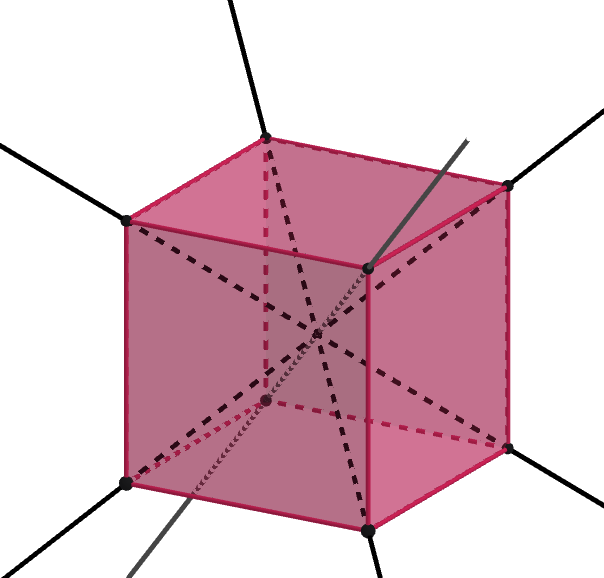
\includegraphics[width=0.6\textwidth]{images/polyeder/raumdiagonalen.png}
        \caption{Drehachsen eines regulären Hexaeders durch gegenüberliegende Ecken ($120^\circ$-Drehungen).}
        \label{fig:drehachsen}
    \end{figure}
    \end{itemize}
    Da diese Achsen nicht identisch sind, kann keine einzelne Gerade unter allen Elementen von $\Omega$ invariant sein. Dies führt zu einem Widerspruch, womit die Irreduzibilität bewiesen ist.
\end{proof}


\subsubsection{Orthogonale Matrizen} \label{sec:orthogonalrotation}
In diesem Abschnitt zeigen wir, dass Matrizen, die eine Drehung im euklidischen Raum beschreiben, stets orthogonale Matrizen sind.

\begin{lemma} \label{lemma:drehungensindorthogonalmatrizen}
    Eine Matrix $R \in \mathbb{R}^{n \times n}$, die eine Drehung repräsentiert, ist eine orthogonale Matrix. Es gilt somit $R^T R = I$, wobei $I$ die Einheitsmatrix bezeichnet.
\end{lemma}

\begin{proof}
    Seien $\vec{v}, \vec{w} \in \mathbb{R}^n$. Eine Drehung ist eine Isometrie; per Definition bleiben unter dieser Transformation zwei Eigenschaften invariant:
\begin{itemize}
    \item Die Längen der Vektoren verändern sich nicht ($\|\vec{v}\| = \|R\vec{v}\|$).
    \item Der Winkel zwischen zwei Vektoren bleibt erhalten.
\end{itemize}
Da eine Drehung somit das Skalarprodukt (und damit Längen und Winkel) erhält, muss für beliebige Vektoren $\vec{v}$ und $\vec{w}$ gelten
\begin{align*}
    (R\vec{v}) \cdot (R\vec{w}) = \vec{v} \cdot \vec{w}.
\end{align*}
Unter Verwendung der Matrixschreibweise für das Skalarprodukt $(\vec{a} \cdot \vec{b} = \vec{a}^T \vec{b})$ erhalten wir:
\begin{alignat*}{2}
    & (R\vec{v})^T (R\vec{w}) &&= \vec{v}^T\vec{w} \\
    \iff & \vec{v}^T R^T R \vec{w} &&= \vec{v}^T\vec{w} \\
    \iff & \vec{v}^T (R^T R) \vec{w} &&= \vec{v}^T I \vec{w}.
\end{alignat*}
Da diese Gleichung für alle Vektoren $\vec{v}, \vec{w} \in \mathbb{R}^n$ erfüllt sein muss, folgt daraus unmittelbar die Matrizengleichung:
\begin{align}
    R^T R = I. \nonumber
\end{align}
\end{proof}

